\RequirePackage[l2tabu,orthodox]{nag}

% TODO: decide if one-sided/two-sided
%\documentclass[headsepline,footsepline,footinclude=false,fontsize=11pt,paper=a4,listof=totoc,bibliography=totoc,BCOR=12mm,DIV=12]{scrbook} % two-sided
%\documentclass[headsepline,footsepline,footinclude=false,oneside,fontsize=11pt,paper=a4,listof=totoc,bibliography=totoc]{scrbook} % one-sided

\documentclass[a4paper,11pt,oneside]{book}

\PassOptionsToPackage{table,svgnames,dvipsnames}{xcolor}

\usepackage[utf8]{inputenc}
\usepackage[T1]{fontenc}
\usepackage[sc]{mathpazo}
\usepackage[american]{babel}
\usepackage[autostyle]{csquotes}
\usepackage[%
  backend=biber,
  url=false,
  style=alphabetic,
  maxnames=4,
  minnames=3,
  maxbibnames=99,
  firstinits,
  uniquename=init]{biblatex} % TODO: adapt bibliography style
\usepackage{graphicx}
\usepackage{scrhack} % necessary for listings package
\usepackage{listings}
\usepackage{lstautogobble}
\usepackage{tikz}
\usepackage{pgfplots}
\usepackage{pgfplotstable}
\usepackage{booktabs}
\usepackage[final]{microtype}
\usepackage{caption}
\usepackage[hidelinks]{hyperref} % hidelinks removes colored boxes around references and links
\usepackage[toc,nonumberlist,acronym]{glossaries} % TODO: remove if glossary not needed
%\usepackage{showframe}


\bibliography{bibliography/literature}


%scrbook
%%%%\setkomafont{disposition}{\normalfont\bfseries} % use serif font for headings
\linespread{1.3} % adjust line spread for mathpazo font

% Settings for glossaries TODO: remove the following block if glossary not needed
\renewcommand{\glsnamefont}[1]{\normalfont\bfseries #1} % use serif font for glossary entry titles
\makeglossaries{}

% Settings for pgfplots
\pgfplotsset{compat=1.9} % TODO: adjust to your installed version
\pgfplotsset{
  % For available color names, see http://www.latextemplates.com/svgnames-colors
  cycle list={CornflowerBlue\\Dandelion\\ForestGreen\\BrickRed\\},
}

% Settings for lstlistings
\lstset{%
  basicstyle=\ttfamily,
  columns=fullflexible,
  autogobble,
  keywordstyle=\bfseries\color{MediumBlue},
  stringstyle=\color{DarkGreen}
}

% Basic information for cover & title page
\newcommand*{\getUniversity}{Technische Universität München}
\newcommand*{\getFaculty}{Department of Informatics}
\newcommand*{\getTitle}{Research and Analysis of Copy Protection Mechanisms for Android Apps, as well as implementing a Sample Application}
\newcommand*{\getTitleGer}{Erforschung und Analyse von Kopierschutzverfahren für Android Apps, sowie Umsetzung in einer Beispielapplikation}
\newcommand*{\getAuthor}{Sebastian Schleemilch}
\newcommand*{\getDoctype}{Master's Thesis in Automotive Software Engineering}
\newcommand*{\getSupervisor}{Prof. Dr. Uwe Baumgarten}
\newcommand*{\getAdvisor}{Nils Kannengießer, M.Sc. }
\newcommand*{\getSubmissionDate}{15.04.2016}
\newcommand*{\getSubmissionLocation}{Munich}
\newcommand*{\Appendixautorefname}{Appendix}
\renewcommand{\texttt}[1]{%
  \begingroup
  \ttfamily
  \begingroup\lccode`~=`/\lowercase{\endgroup\def~}{/\discretionary{}{}{}}%
  \begingroup\lccode`~=`[\lowercase{\endgroup\def~}{[\discretionary{}{}{}}%
  \begingroup\lccode`~=`.\lowercase{\endgroup\def~}{.\discretionary{}{}{}}%
  \catcode`/=\active\catcode`[=\active\catcode`.=\active
  \scantokens{#1\noexpand}%
  \endgroup
}
\newcommand{\code}[1]{\texttt{#1}}

% TODO: add custom commands etc.


% TODO: remove if glossary not needed
%\newglossaryentry{computer}
{
  name=computer,
  description={is a machine that\ldots}
}

\newacronym{app}{App}{Short term for (mobile) installable application}
\newacronym{gui}{GUI}{Graphical User Interface}
\newacronym{hal}{HAL}{Hardware Abstraction Layer}
\newacronym{jni}{JNI}{Java Native Interface}
\newacronym{dvm}{DVM}{Dalvik Virtual Machine}
\newacronym{glibc}{GLIBC}{GNU C Library}
\newacronym{art}{ART}{Android Runtime}
\newacronym{api}{API}{Application Interface}
\newacronym{jvm}{JVM}{Java Virtual Machine}
\newacronym{vm}{VM}{Virtual Machine}
\newacronym{dex}{DEX}{Dalvik Executable}
\newacronym{jit}{JIT}{Just-In-Time}
\newacronym{aot}{AOT}{Ahead-Of-Time}
\newacronym{ndk}{NDK}{Native Development Kit}
\newacronym{jar}{JAR}{Java Library}
\newacronym{apk}{APK}{Android Application Package}
\newacronym{os}{OS}{Operating System}
\newacronym{adb}{ADB}{Android Debug Bridge}
\newacronym{zip}{ZIP}{Zipper file format}
\newacronym{ui}{UI}{User Interface}
\newacronym{ipc}{IPC}{Inter Process Communication}
\newacronym{cpu}{CPU}{Central Processing Unit}
\newacronym{jdk}{JDK}{Java Development Kit}
\newacronym{pm}{pm}{Package Manager}
\newacronym{odex}{ODEX}{Optimized Dalvik Executable}
\newacronym{elf}{ELF}{Executable Linking Format}
\newacronym{uid}{UID}{User Identification Number}
\newacronym{gid}{GID}{Group Identification Number}
\newacronym{oop}{OOP}{Object Oriented Programming}
\newacronym{mime}{MIME}{Internet Media Type}
\newacronym{tis}{TIS}{Tool Interface Standards}
\newacronym{ide}{IDE}{Integrated Development Environment}
\newacronym{pid}{PID}{Process ID}
\newacronym{ppid}{PPID}{Parent Process ID}
\newacronym{aosp}{AOSP}{Android Open Source Project}



\begin{document}

\begin{titlepage}
  % HACK for two-sided documents: ignore binding correction for cover page.
  % Adapted from Markus Kohm's KOMA-Script titlepage=firstiscover handling.
  % See http://mirrors.ctan.org/macros/latex/contrib/koma-script/scrkernel-title.dtx,
  % \maketitle macro.
  \oddsidemargin=\evensidemargin\relax
  \textwidth=\dimexpr\paperwidth-2\evensidemargin-2in\relax
  \hsize=\textwidth\relax

  \centering

  \vspace{0mm}
  
\includegraphics[width=40mm]{logos/tum}

  \vspace{10mm}
  {\huge\MakeUppercase{\getFaculty{}}}\\
  %\vspace{5mm}
  {\large\MakeUppercase{\getUniversity{}}}\\

  \vspace{40mm}
  {\Large \getDoctype{}}

  \vspace{30mm}
  {\huge\bfseries \getTitle{}}

  \vspace{30mm}
  {\LARGE \getAuthor{}}

  \vspace{30mm}
  
\includegraphics[width=20mm]{logos/faculty}
\end{titlepage}


\frontmatter{}
\begin{titlepage}
  \centering

  \vspace{40mm}
  
\includegraphics[width=40mm]{logos/tumBlue}

  \vspace{10mm}
  {\huge\MakeUppercase{\getFaculty{}}}\\

  %\vspace{5mm}
  {\large\MakeUppercase{\getUniversity{}}}\\

  \vspace{20mm}
  {\Large \getDoctype{}}

  \vspace{15mm}
  {\huge\bfseries \getTitle{}}

  \vspace{15mm}
  {\huge\bfseries \getTitleGer{}}

  \vspace{20mm}
  \begin{tabular}{l l}
    Author: & \getAuthor{} \\
    Supervisor: & \getSupervisor{} \\
    Advisor: & \getAdvisor{} \\
    Submission Date: & \getSubmissionDate{} \\
  \end{tabular}

  \vspace{20mm}
  
\includegraphics[width=20mm]{logos/facultyBlue}
\end{titlepage}

\thispagestyle{plain}
\vspace*{0.8\textheight}
\noindent
I confirm that this master's thesis is my own work and I have documented all sources and material used.

\vspace{20mm}
\noindent
\getSubmissionLocation{}, \getSubmissionDate{} \hspace{5cm} \getAuthor{}


%\addcontentsline{toc}{chapter}{Acknowledgments}
\thispagestyle{empty}

\vspace*{2cm}

\begin{center}
{\usekomafont{section} Acknowledgments}
\end{center}

\vspace{1cm}

%TODO: Acknowledgments

\cleardoublepage{}

\chapter{\abstractname}




\microtypesetup{protrusion=false}
\tableofcontents{}
\microtypesetup{protrusion=true}

\printglossaries{}


\mainmatter{}
\pagestyle{fancy}
\fancyhead{}
\fancyhead[C]{\slshape \leftmark}
\fancyfoot[C]{\thepage}


%\chapter{Introduction}\label{chapter:introduction}

\section{Section}
Citation test~\parencite{latex}.

\subsection{Subsection}
See~\autoref{fig:sample}.

\begin{figure}[htb]
  \centering
  
\includegraphics{logos/tum}
  \caption[Example figure]{An example for a figure.}\label{fig:sample}
\end{figure}

\section{Section}

See~\autoref{tab:sample}, \autoref{fig:sample-drawing}, \autoref{fig:sample-plot}, \autoref{fig:sample-listing}.

\begin{table}[htb]
  \caption[Example table]{An example for a simple table.}\label{tab:sample}
  \centering
  \begin{tabular}{l l l l}
    \toprule
      A & B & C & D \\
    \midrule
      1 & 2 & 1 & 2 \\
      2 & 3 & 2 & 3 \\
    \bottomrule
  \end{tabular}
\end{table}

\begin{figure}[htb]
  \centering
  % This should probably go into a file in figures/
  \begin{tikzpicture}[node distance=3cm]
    \node (R0) {$R_1$};
    \node (R1) [right of=R0] {$R_2$};
    \node (R2) [below of=R1] {$R_4$};
    \node (R3) [below of=R0] {$R_3$};
    \node (R4) [right of=R1] {$R_5$};

    \path[every node]
      (R0) edge (R1)
      (R0) edge (R3)
      (R3) edge (R2)
      (R2) edge (R1)
      (R1) edge (R4);
  \end{tikzpicture}
  \caption[Example drawing]{An example for a simple drawing.}\label{fig:sample-drawing}
\end{figure}

\begin{figure}[htb]
  \centering

  \pgfplotstableset{col sep=&, row sep=\\}
  % This should probably go into a file in data/
  \pgfplotstableread{
    a & b    \\
    1 & 1000 \\
    2 & 1500 \\
    3 & 1600 \\
  }\exampleA
  \pgfplotstableread{
    a & b    \\
    1 & 1200 \\
    2 & 800 \\
    3 & 1400 \\
  }\exampleB
  % This should probably go into a file in figures/
  \begin{tikzpicture}
    \begin{axis}[
        ymin=0,
        legend style={legend pos=south east},
        grid,
        thick,
        ylabel=Y,
        xlabel=X
      ]
      \addplot table[x=a, y=b]{\exampleA};
      \addlegendentry{Example A};
      \addplot table[x=a, y=b]{\exampleB};
      \addlegendentry{Example B};
    \end{axis}
  \end{tikzpicture}
  \caption[Example plot]{An example for a simple plot.}\label{fig:sample-plot}
\end{figure}

\begin{figure}[htb]
  \centering
  \begin{tabular}{c}
  \begin{lstlisting}[language=Java]
    SELECT * FROM tbl WHERE tbl.str = "str"
  \end{lstlisting}
  \end{tabular}
  \caption[Example listing]{An example for a source code listing.}\label{fig:sample-listing}
\end{figure}

asdfasdfasdffffffffffffffdasdfasdfasdf
asdfasdfasdfffffffffffasdfasdfasdfsadf
asdfasdfasdffffffffffffffdasdfasdfasdf
asdfasdfasdfffffffffffasdfasdfasdfsadf
asdfasdfasdffffffffffffffdasdfasdfasdf
asdfasdfasdfffffffffffasdfasdfasdfsadf
asdfasdfasdffffffffffffffdasdfasdfasdf
asdfasdfasdfffffffffffasdfasdfasdfsadf
asdfasdfasdffffffffffffffdasdfasdfasdf
asdfasdfasdfffffffffffasdfasdfasdfsadf
asdfasdfasdffffffffffffffdasdfasdfasdf
asdfasdfasdfffffffffffasdfasdfasdfsadf
asdfasdfasdffffffffffffffdasdfasdfasdf
asdfasdfasdfffffffffffasdfasdfasdfsadf

\chapter{Android Status Quo}\label{chapter:android_status_quo}

\section{Popularity of Android}
Android is an operating system by Google,
designed for mobile devices. Version 1.0 was released
in 2008. With a remarkable market share of 82.8\%
it has grown into the most important mobile operating system
followed by Apple's iOS with 13.9\% and Microsoft's Windows
Phone with 2.6\%. See \parencite{Idc15} for a full list
of mobile operating system market shares. While the smartphone
market is still growing, Android did also attach to new
rising platforms like wearables, TV's, cars and general
embedded devices.




\chapter{Android Basics}\label{chapter:android_basics}

\section{Android Architecture}
To provide copy protection mechanisms for Android apps,
of course a deep understanding of the Android system itself
is necessary. As mentioned in~\autoref{chapter:android_status_quo},
Android is built on the Linux kernel. Android does provide not
only shell binaries (Linux kernel) but also a GUI environment
as well as predefined frameworks and a complete environment
for developers to write apps in the Java programming language.
That's why Android is considered to be a ``full software stack''
~\parencite{levin}. Although it's built on Linux,
Google did modify the Linux kernel to their need.
As a result, the Android kernel differs
incompatibly with the Linux kernel since version 2.6.27.

The difference at kernel-level is not massive compared to
the differences at user-mode where Android does have entirely new
components, namely:

\begin{itemize}
\item Dalvik Runtime including the Dalvik Virtual Machine (DVM)
respectively the Android Runtime (ART) since Android version > 5.0.
\item The Bionic C-Library instead of the GNU C Library (GlibC)
\item Hardware Abstraction Layer (HAL)
\item Java Native Interface (JNI)
\item Android specific frameworks
\end{itemize}

\autoref{fig:androidvslinux} visually summarizes the difference
between Android and Linux.

\begin{figure}[htb]
  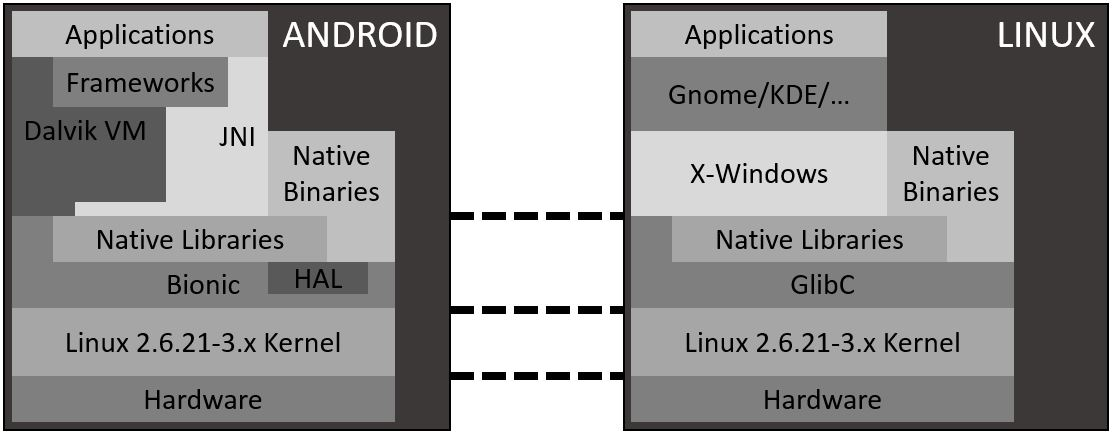
\includegraphics[width=\textwidth]{figures/androidvslinux}
  \caption[Android vs Linux]{Android and Linux comparison
  ~\parencite{levin}}
  \label{fig:androidvslinux}
\end{figure}

The Android specific frameworks are the core work that makes Android
special. They simplify the creation process of applications massively.
Developers can use the high level language Java rather than developing
in C/C++. Additionally, there is a rich set of APIs to solve most of
programmers everyday problems.

In order to get Java programs run on Android, the DVM is introduced
which is quite similar to a Java Virtual Machine (JVM).
The DVM provides an interface between the operating system and
the Java application world, after all the execution of Java programs.
The difference between DVM and JVM is the alternative form of bytecode
which gets executed in the VM. DVM is optimized for mobile devices
in terms of efficiency and sharing memory and is using the
Dalvik Executable format (DEX) as bytecode which is still device
independent ~\parencite{levin}.

With Android version 5.0, Google did introduce ART.
The prior Dalvik runtime does use Just-In-Time (JIT) compiling
where executable machine code is created not until runtime.
ART on the other hand does use Ahead-Of-Time (AOT) compilation
which compiles an app to machine code at installation time.
The reason for JIT in the first place were among other things
storage limitations of mobile devices at the time Android was released
~\parencite{levin}. As a result, the ART apps installation time
is increased as well as the required storage space as a tradeoff
to the app startup and runtime performance. As we will see,
Dalvik is still very much deep-seated in Android even under ART.

The JNI provides an opportunity to write Java programs with embedded
native processor specific code to escape from the VM world
such as direct hardware access.
It is mostly used to optimize the performance for apps (e.g games)
or to hinder reverse engineering of the application code.
Google does provide an Native Development Kit (NDK) to help
developers creating native libraries ~\parencite{ndk}.

Bionic is the Android corresponding GlibC library which was created
for license and simplicity reasons. Overall, it is more lightweight
than the GlibC and well adapted for Android.

Since Android is like to run on a great variety of devices,
it has to support a great amount of different hardware.
The HAL standardizes the interface and allows hardware vendors
to implement their own drivers ~\parencite{levin}.

\section{Android Apps}

\chapter{Copy Protection Status Quo}
\label{chapter:copy_protection_status_quo}

Like introduced in \autoref{chapter:android_status_quo} there
are different goals of copy protection mechanisms starting from
preventing reverse code engineering to protect intellectual property
and reaching to hinder patching to get prohibited access.
The common denominator of those goals is the protection of
the DEX file of every app. A variety of tools do exist that
are able to transform DEX into different readable formats,
modify it and repack it again since the DEX contains
a lot of meta data for its contents (classes, methods, \ldots)
\parencite{dex}.


\section{DEX Dissassembly and Repackaging}
Generally there do exist two possible outcomes of DEX disassembling
- Java code (\code{*.java}) and Smali code (\code{*.smali}).
Since the DEX format is more or less just a different mapping of a
JAR and its containing \code{.class} files, the transition to JAR
is quite simple \parencite{dvminternals}. A tool that is able to
perform this step is ``dex2jar'' \parencite{dex2jartool}.
Along with this JAR, standard Java decompiler like ``JD-GUI''
\parencite{jdtool} can be used to produce the \code{*.java} source code.
If the \code{*.java} is supposed to change and repacked, it can
be again compiled into JAR with Oracle's ``javac'' \parencite{javactool}
followed by Googles ``dx'' tool \parencite{dxtool}
to produce the manipulated DEX.

The alternative way is the use of ``smali/baksmali'' tool
\parencite{smalitool} which is a direct assembler and disassembler
for DEX files rather than taking the Java code detour. There is also
a tool included that can convert the ODEX back to DEX.

Overall, the dissassembly of unchanged DEX is quite easy and is shown
as a concluding overview in \autoref{fig:dex_disassembly}

Therefore several countermeasures were established which are
described in the following sections.

\begin{figure}[htb]
  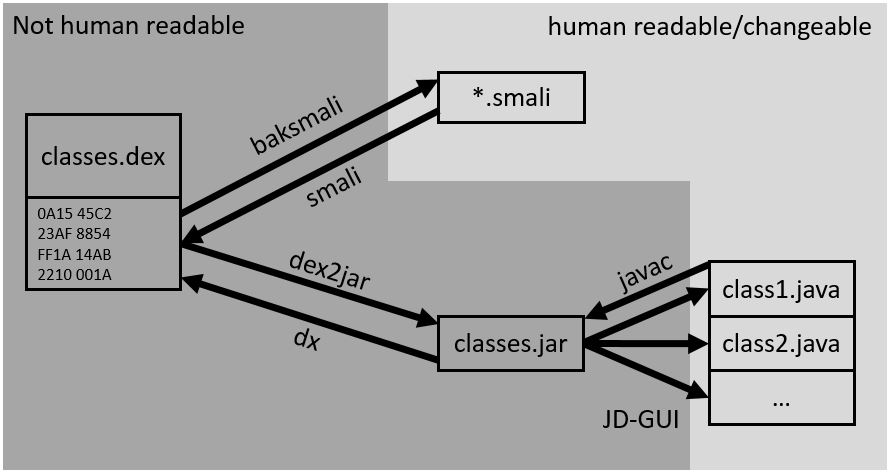
\includegraphics[width=\textwidth]{figures/dex_disassembly}
  \caption[DEX Assembly/Disassembly]{DEX Assembly/Disassembly}
  \label{fig:dex_disassembly}
\end{figure}


\section{Obfuscation Techniques}
Obfuscation in the context of copy protection for application
is generally the term for hardening an application against
reverse code engineering techniques. It can be achieved by different methods
that can be seperated in two main groups, static and dynamic obfuscation.
Static means that the obfuscation technique is applied to code units (source
code, binaries, ...) while the application is not executed. Therefore an
attacker could possibly successful analyze the application without executing it
if he manages to break this obfuscation. Applications that are dynamically
obfuscated on the other hand, are much harder to analyze since the behavior
of the application is not decided until its execution. An attacker needs to connect to the process of the application followed by a just in time inspection.

It does follow a list of common static and dynamic obfuscation techniques
for Android applications.

\subsection{Static}
\subsubsection{Common Source Code Obfuscation}
The most common way of harden source code is to remove any kind of meta data
that has been added during the development process. Means destroying/modifying
information that originally was present in the source code.
This technique can be applied at different layers, \code{.java}, \code{.class} and the final \code{.dex} in case of Android.
Among other things they consist of renaming
classes, variables, functions, irreducable code insertion,
artificial parallelization, method inlining/outlining, unrolling
loops, encoding strings, changing the control flowand so on to confuse code analysts but always keeping its original behavior.

Popular tools for that purpose are Google's ``ProGuard''
\parencite{proguardtool} which is included in the Android build system and
can be enabled easily as well as``DexGuard'' by GuardSquare
\parencite{dexguardtool}. ``ProGuard'' does
operate on source code level where ``DexGuard'' operates on DEX.
Since the first unit of Android applications is Java code, classical Java
obfuscators also can be used.

\subsubsection{Junk-Byte-Insertion}
Junk-Byte-Insertion's goal is to confuse static analyzing
disassembling tools. It does work for tools with the
``linear sweep'' method to analyze a file. That means
the tools are processing every instruction from the entrypoint
till the end without interpreting them (e.g. not following jumps).
That examining technique can be exploited to break the disassembling
procedure. Let's assume we do have the code snippet of
\autoref{fig:junk_byte_listening}
on source code level.

\begin{figure}[htb]
  \centering
  \begin{tabular}{c}
  \begin{lstlisting}[language=Java]
    if (false) {
        0x12 0x34 0x56
    } else {
        proceedProgram()
    }
  \end{lstlisting}
  \end{tabular}
  \caption[Junk-Byte-Insertion]{Junk-Byte-Insertion Example}
  \label{fig:junk_byte_listening}
\end{figure}

Cause of the if-condition, the \code{insertBreakingBytes()} method is never
reached. Since ``linear sweep'' does not perform jumps, the analyzing tool
is trying to revert those bytes into source code. By choosing a specific
sequence of bytes, the transformation will fail.

Enhanced tools will use the ``recursive traversal'' technique to analyze a
file which is capable of detecting dead branches like in the example above.
These tools also may be tricked by choosing a more complicated condition for
if-conditions that can only be evaluated at runtime and therefore the
whole conditional branch (including the breaking byte sequence) would also be evaluated.
\parencite{lvl_imp}.

\subsection{Dynamic}
\subsubsection{Hidden Methods Invocation}
\subsubsection{Dynamic Code Loading}
\subsubsection{Self Modifying Code}





% TODO: add more chapters here

\appendix{}
 % TODO: remove if glossary not needed
\glsaddall{} % add all defined terms to glossary, even if not referenced in text
\microtypesetup{protrusion=false}
\listoffigures{}
\listoftables{}
\microtypesetup{protrusion=true}
\printbibliography{}

\end{document}
